%\noindent
\justifying
\setlength{\parskip}{1em}

This chapter discusses the implementation of the \ac{CycleGAN} and Classifiers. In this thesis, classifiers are used to determine the domain gap between the distributions. Also, they are used to evaluate the quality of images generated by the \ac{CycleGAN}. How the classifiers are being used to analyze the domain gap between distributions will be discussed in-depth in chapter Evaluation \ref{evaluation}. In section \ref{DatasetPreparation} dataset preparation is described. The architecture of \ac{CycleGAN} and Classifiers discussed in section \ref{NetworkArchitecture}. The training details of \ac{CycleGAN} and Classifiers described in \section{Training Details}. The experiments are visualized using Tensorboard\footnotemark. TensorBoard is a tool that provides the visualization needed for machine learning research and experiments. The neural networks implemented in this thesis using Python, Keras APIs, and TensorFlow library\cite{tensorflow2015-whitepaper}. The reference code for the \ac{CycleGAN} is available \href{https://keras.io/examples/generative/cyclegan/}{here}. All of the neural networks are trained upon GPUs (Graphics Processing Units) like Nvidia Tesla T4 and Tesla V100-SXM2.

\footnotetext{\url{https://www.tensorflow.org/tensorboard} last access: 04.05.2021}


\section{Dataset Preparation}\label{DatasetPreparation}

\begin{figure}[H]
        \begin{center}
    	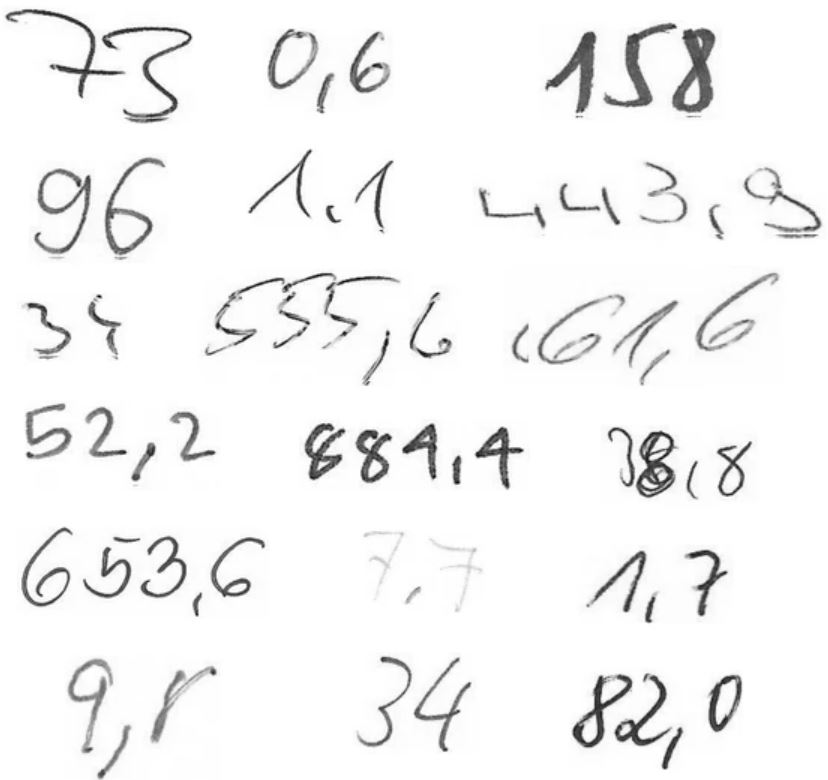
\includegraphics[scale=0.45]{images/keinwifi.JPG}
	    \caption[Examples of Handwritting Crops from the Handwritting Number Dataset.]{Examples of Handwritting Crops from Handwritting Number Dataset. (Figure reproduced from elevait GmbH \& Co. KG with permission.)}
	    \label{fig:keinwifi}
	    \end{center}
\end{figure}


The dataset preparation is one of the vital aspects of training any neural network. Bad quality data leads to a poor generalization of neural networks. There are ten types of documents that were considered to work with this image-to-image translation application. Hence, the \ac{CycleGAN} is trained using a stash of synthetic document images and real document images. Around 100,000 synthetic document images in the source domain and the same number of real document images in the target domain. The synthetic document images are generated using unfilled form image (figure \ref{fig:EmptyForm}) and handwritten crops (figure \ref{fig:keinwifi}). The process of inserting handwritten crops on empty templates can be visualized in figure \ref{fig:InsertHandwrittenCrops}. Each unfilled form image is filled with the help of provided bounding box annotations \cite{lin2015microsoft}. For each class of unfilled form image 10,000, synthetic document images are created. As mentioned earlier, 100,000 synthetic document images are created in total. The same created 100,000 synthetic document images are used while training \ac{CycleGAN}. Just they are stashed at the same location collectively. The created 100,000 synthetic document images were also faxified and a faxified dataset of 100,000 images is created. It has the same structure as synthetic document images, 10 classes, and each class has 10,000 images. The faxification process uses several image transformations to make a clean gray-scale image look like it was sent via fax. A sample faxified image can be seen in figure \ref{fig:FaxifiedImage}. The faxification process is described briefly in Section \ref{trainingfaxifiedclassifier}. Also, the faxification can be visualized in figure \ref{fig:FaxificationProcess}. In the table \ref{table:datasets} the number of samples in each dataset is mentioned. For testing, around 1162 annotated real document images are used. This testing dataset is used to evaluate the performance of the classifiers trained upon different data distributions like synthetic document images, faxified document images, and \ac{CycleGAN} generated document images. Basically, testing dataset is significant to understand the domain gap between real data distribution and remaining data distributions. In the table \ref{table:testdataset} the number of samples in each class in the test dataset is mentioned. The testing dataset is unbalanced. The datasets used in this thesis can not be cited or published because they are not open for public use.

\begin{figure}[H]
        \begin{center}
	    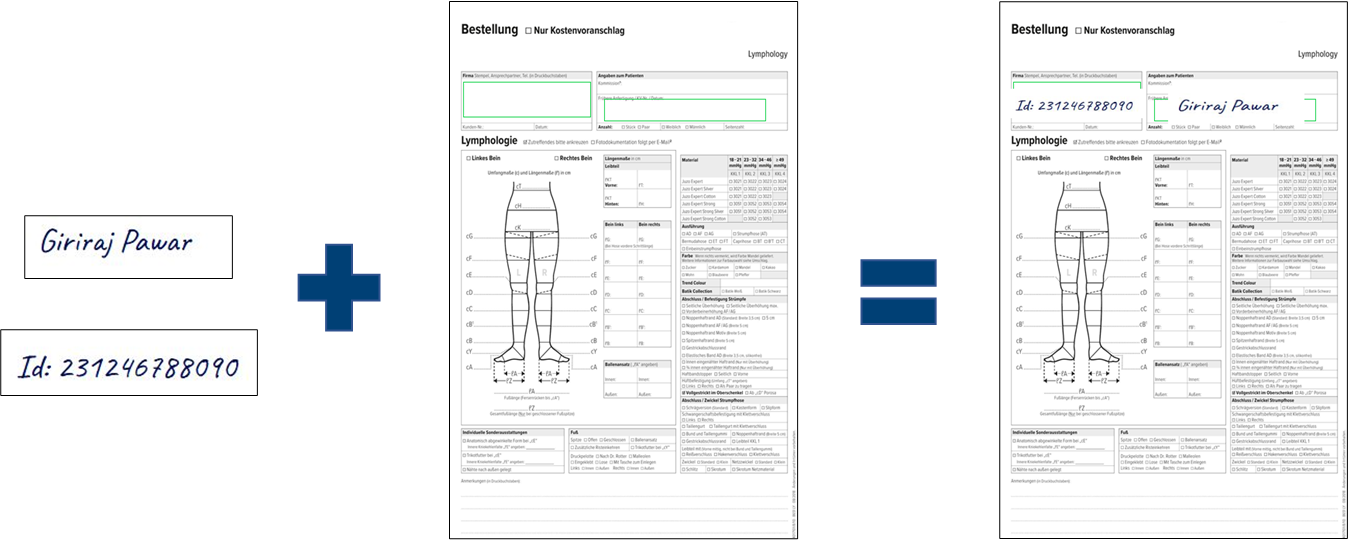
\includegraphics[scale=0.40]{images/InsertHandwrittenCrops.png}
	    \caption{Inserting Handwritten Crops in Empty Form Templates.}
	    \label{fig:InsertHandwrittenCrops}
	    \end{center}
\end{figure}


\begin{center}
    \begin{table}[H]
    \begin{center}
    \begin{tabular}{||c c||} 
    \hline
    \textbf{Datasets} & \textbf{Size (Number of Images)}\\ [0.5ex] 
    \hline\hline
    Synthetic Document Images & 100,000 \\ 
    \hline
    Real Document Images & 100,000 \\
    \hline
    Faxified Document Images & 100,000 \\
    \hline
    Annotated Real Document Images (Used for testing) & 1162 \\
    \hline
    \end{tabular}
    \end{center}
    \caption{Size of Datasets used for training \ac{CycleGAN} and Classifiers.}
    \label{table:datasets}
    \end{table}
\end{center}

\begin{center}
    \begin{table}[H]
    \begin{center}
    \begin{tabular}{||c c||} 
    \hline
    \textbf{Classes} & \textbf{Size (Number of Images)}\\ [0.5ex] 
    \hline\hline
    DE\_LY\_Arm\_2020-01 & 44 \\ 
    \hline
    DE\_LY\_Bein\_2018-08 & 47 \\
    \hline
    DE\_LY\_Bein\_2019-01 & 50 \\
    \hline
    DE\_LY\_Bein\_2019-07&  60\\
    \hline
    DE\_LY\_Bein\_2020-01&  624\\
    \hline
    DE\_LY\_Bein\_2020-03&  128\\
    \hline
    DE\_LY\_Hand\_2020-01&  16\\
    \hline
    DE\_PH\_Bein\_2018-09&  22\\
    \hline
    DE\_PH\_Bein\_2019-02&  28\\
    \hline    
    DE\_PH\_Bein\_2020-01&  143\\
    \hline    
    \end{tabular}
    \end{center}
    \caption[Number of Images in each Class of Annotated Real Document Images Dataset.]{Number of Images in each Class of Annotated Real Document Images Dataset.}
    \label{table:testdataset}
    \end{table}
\end{center}



\begin{figure}[H]
        \begin{center}
	    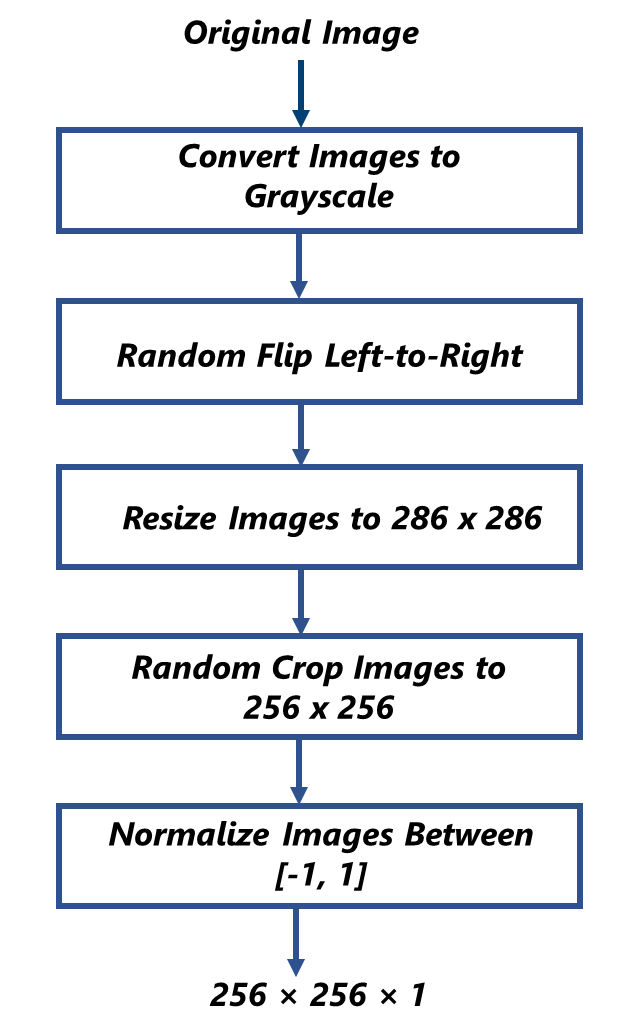
\includegraphics[scale=0.40]{images/Preprocessing.png}
	    \caption[Steps involved in preprocessing of training images of \ac{CycleGAN}.]{Steps involved in preprocessing of training images of \ac{CycleGAN}.}
	    \label{fig:Preprocessing}
	    \end{center}
\end{figure}


\section{Network Architecture}\label{NetworkArchitecture}

\subsection{\ac{CycleGAN}}

Johnson et al.\cite{johnson2016perceptual} proposed the architecture of \ac{CycleGAN}. In which the generator has three sequences of blocks one is downsampling, transformation, and upsampling. The sequence of 2 downsampling convolutional blocks encode the $256 \times 256 \times 1$ grayscale input image, 9 \ac{ResNet} convolutional blocks to transform the image, and a 2 upsampling convolutional blocks to generate the output image of the same dimension as the input image. The reason behind using residual blocks is it resolves the vanishing gradient problem in deep neural networks. The discriminator classifier network is designed using PatchGAN architecture \cite{isola2018imagetoimage} \cite{li2016precomputed}. The PatchGAN discriminator is simply a \ac{CNN}. The major difference between the PatchGAN discriminator and General \ac{GAN} discriminator is, \ac{GAN} discriminator maps input image to the scalar output, which represents image being real to fake. But, the PatchGAN discriminator maps the input image to $N \times N$ array of outputs, where each element in an output array represent a patch in an input image being real or fake. Basically, the PatchGAN discriminator penalizes structure at the scale of local image patches and attempts to classify if each $M \times M$ patch in an image is real or fake.

Johnson et al. \cite{johnson2016perceptual} have provided naming conventions to define the architecture of generator and discriminator used in \ac{CycleGAN}. {\fontfamily{qcr}\selectfont c7s1-k} denotes a $7 \times 7$ Convolution-InstanceNormlization-ReLU layer with $k$ filters and stride 1. The downsampling block {\fontfamily{qcr}\selectfont dk} denoted by a $3 \times 3$ Convolution-InstanceNormlization-ReLU layer with $k$ filters and stride 2. To reduce artifacts reflection padding is used. {\fontfamily{qcr}\selectfont Rk} denotes a single residual block that has two $3 \times 3$ convolutional layers with the same number of filters $k$ on both layers and stride 1. The upsampling block {\fontfamily{qcr}\selectfont uk} denoted a $3 \times 3$ TransposedConvolution-InstanceNormlization-ReLU layer with $k$ filters and stride 2. The complete generator network with 9 residual blocks can be decribed as: {\fontfamily{qcr}\selectfont c7s1-64, d128, d256, R256, R256, R256, R256, R256, R256, R256, R256, R256, u128, u64, c7s1-1}. The last layer {\fontfamily{qcr}\selectfont c7s1-1} denotes a $7 \times 7$ Convolution layer with 1 filter and stride 1. Next, the final output is followed by a tanh activation function (figure \ref{fig:ActivationFunctions}). All of the layers in the generator can be seen in figure \ref{fig:generator}.


\begin{center}
\begin{table}[H]
    \begin{center}
    \begin{tabular}{p{0.15\linewidth} p{0.10\linewidth} p{0.10\linewidth} p{0.10\linewidth} p{0.10\linewidth}} 
        \toprule
         Operation Layer & Number of Filters & Size of Each Filter & F1-score & Support\\[0.0ex] 
        \midrule
      
        \bottomrule
    \end{tabular}
    \caption[]{}
    \label{table:discriminatorArchitecture}
    \end{center}
\end{table}
\end{center}

\begin{figure}[H]
        \begin{center}
	    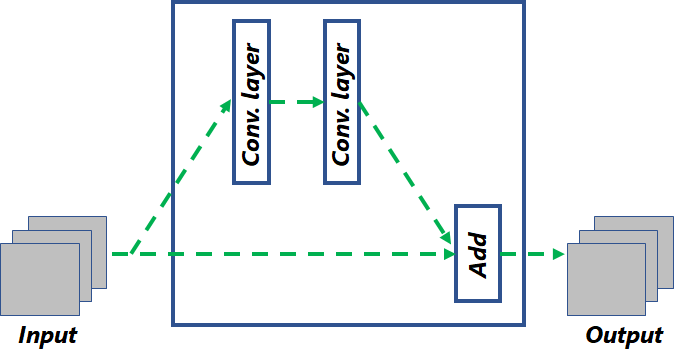
\includegraphics[scale=0.50]{images/resnetBlocks.png}
	    \caption[Illustration of ResNet Blocks in \ac{CycleGAN} Generator Architecture.]{Illustration of ResNet Blocks in \ac{CycleGAN} Generator Architecture.}
	    \label{fig:resnetBlock}
	    \end{center}
\end{figure}


The discriminator uses $70 \times 70$ PatchGAN classfier architecture \cite{isola2018imagetoimage}. It is also called a Markovian discriminator \cite{li2016precomputed}. {\fontfamily{qcr}\selectfont Ck} denotes a $4 \times 4$ Convolution-InstanceNormalization-LeakyReLU layer with $k$ filters and stride 2. Leaky ReLUs with a slope of 0.2 are used. Instance Normalization is not used for the first {\fontfamily{qcr}\selectfont C64} layer. After the last layer {\fontfamily{qcr}\selectfont C512}, the convolution operation is applied with filter 1 to produce an output of depth 1 using $4 \times 4$ kernel and stride 1. The discriminator network can be described as: {\fontfamily{qcr}\selectfont C64-C128-C256-C512}. All of the layers in the discriminator can be seen in figure \ref{fig:discriminator}. For more information on the architectures of generators and discriminators, this Github \href{https://github.com/jcjohnson/fast-neural-style}{repository} can be referred to.

\begin{center}
\begin{table}[H]
    \begin{center}
    \begin{tabular}{p{0.10\linewidth} p{0.10\linewidth} p{0.10\linewidth} p{0.10\linewidth} p{0.10\linewidth}} 
        \toprule
         Operation Layer & Number of Filters & Size of Each Filter\\[0.0ex] 
        \midrule
      
        \bottomrule
    \end{tabular}
    \caption[]{}
    \label{table:discriminatorArchitecture}
    \end{center}
\end{table}
\end{center}



\subsection{Classifier}

The classifier used to determined the domain gap between data distributions is a \ac{CNN}. The classifier architecture is simplistic (figure \ref{fig:ClassifierArchitectureBlocks}). It has just Two Convolution Layers, One Max Pooling Layer, and One Dropout Layer. The architecture of classifier can be preciously visualised in figure \ref{fig:ClassifierArchitecture}. 

\begin{center}
\begin{table}[H]
    \begin{center}
    \begin{tabular}{p{0.22\linewidth} p{0.10\linewidth} p{0.10\linewidth} p{0.10\linewidth} p{0.10\linewidth}} 
        \toprule
        Operation Layer & Number of Filters & Size of Each Filter\\[0.0ex] 
        \midrule
      
        \bottomrule
    \end{tabular}
    \caption[]{}
    \label{table:ClassifierArchitecture}
    \end{center}
\end{table}
\end{center}


\section{Training Details}


\subsection{CycleGAN}
One of the major challenges of the implementation part was designing an efficient input pipeline. The developed image-to-image translation application and classifiers are trained using 100,000 images. Loading such a large dataset is a tedious and time-consuming job but TensorFlow has provided wonderful APIs like \href{https://www.tensorflow.org/guide/data}{tf.data} to load large dataset spontaneously. To learn more about how to load large dataset efficiently in TensorFlow refer this \href{https://www.tensorflow.org/tutorials/load_data/images}{Tutorial}. Two techniques from recent works are applied to stabilize \ac{CycleGAN} model training procedure. First, for $ $ (equation 1), we replace the negative log likelihood
objective by a least-squares loss [


The \ac{CycleGAN} is trained from scratch, with a learning rate of 0.0002. In practice, the objective is divided by 2 while optimizing discriminator (equations \ref{lsgan1} and \ref{lsgan4}), which slows down the rate at which discriminator learns, relative to the rate of generator.  Weights are initialized from a Gaussian distribution with mean ($\mu$) 0 and standard deviation ($\sigma$) 0.02. Images used for the training \ac{CycleGAN} are converted into grayscale. Also, random mirroring and random jittering is applied. In random mirroring, the image is randomly flipped horizontally i.e. left to right. In random jittering, the image is resized to $286 \times 286$ and then randomly cropped to $256 \times 256$. As mentioned in the paper \cite{zhu2020unpaired}, random jittering and mirroring applied to the training dataset. These are some of the image augmentation techniques that avoids overfitting. These are some of the image augmentation techniques that avoid overfitting. Lastly, the images are normalized in the range of $[-1, 1]$. 



The \ac{CycleGAN} is trained for 20 epochs and all the individual models like Forward Generator $G$, Backward Generator $F$, Discriminator $D_Y$, and Discriminator $D_X$ are saved as checkpoints at the end of every epoch. 



\subsection{Classifier}
The images used to train and test the classifiers were also applied with random mirroring and random jittering after converting the image to grayscale. The size of the images is $256 \times 256 \times 1$. Also, the images are normalized in the range of $[-1, 1]$. The classifier architecture can be visualized in figure \ref{fig:ClassifierArchitectureBlocks}. The pre-processing process can be seen in figure \ref{fig:Pre-processingSteps}. The classifier trained using 80\% data and 20\% data used for validation. Subsequently, the performance of the classifiers evaluated using real test document images dataset.













































































%%%%%%%%%%%%%%%%%%%%%%%%%%%%%%%%%%%%%%%%%%%%%%%%%%%%%%%%%%%%%%%%%%%%%%%%%%%%%%%%%%%%%%%%%%%%%%%%%%%

%In the faxification process, several image transformations are applied to the images randomly means the output images produced during this process are random. Transformations like rotation, brightness difference, dithering \cite{8580565} are visible in the above image after the faxification process. The dithering is the process of applying noise intentionally in the images.


\begin{comment}
\begin{figure}[H]
        \begin{center}
    	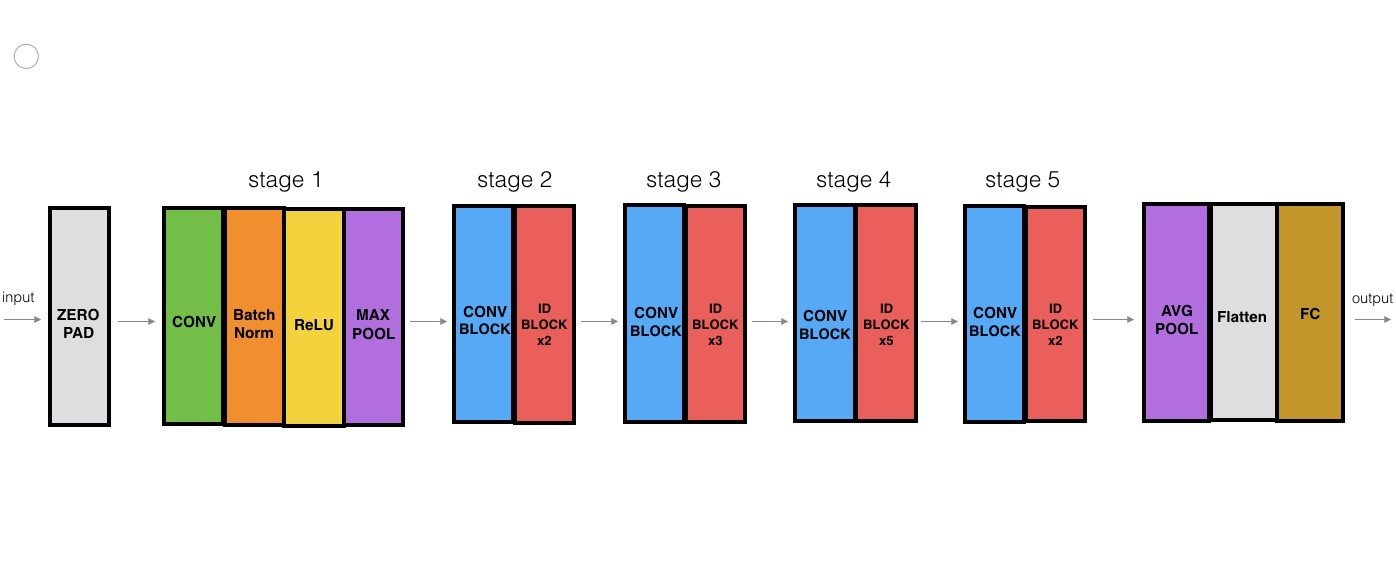
\includegraphics[scale=0.43]{images/ResNet50_1.jpg}
	    \caption[ResNet-50 Classifier Architecture.]{ResNet-50 Classifier Architecture.\footnotemark}
	    \label{fig:ResNet50}
	    \end{center}
\end{figure}
\footnotetext{\url{https://github.com/priya-dwivedi/Deep-Learning/blob/master/resnet_keras/Residual_Networks_yourself.ipynb} last access: 04.05.2021}

\begin{figure}[H]
        \begin{center}
	    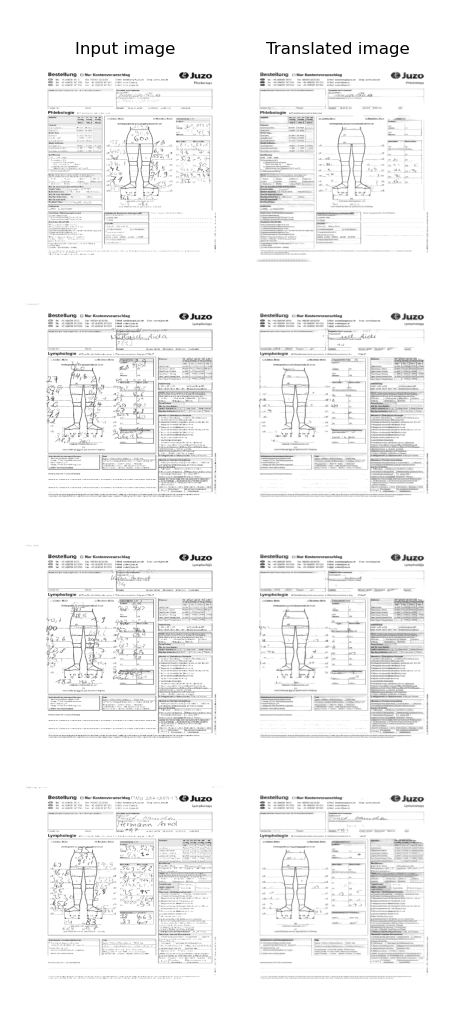
\includegraphics[scale=0.60]{images/CycleGAN_Generated_Images_3_5.png}
	    \caption{\ac{CycleGAN} transalated images.}
	    \label{fig:GeneratedImages}
	    \end{center}
\end{figure}


\end{comment}

\begin{comment}
\begin{figure}[H]
      \centering
      \hspace*{-0.75cm}
      \begin{tikzpicture}
        \node[rotate=0,minimum width=4.5cm] (input) at (0,11.25) {\small{Original Image}};
        \node[conv,rotate=0,minimum width=4.5cm] (Grayscale) at (0,10) {\small{Convert Images to Grayscale}};
        \node[conv,rotate=0,minimum width=4.5cm] (Randomflip) at (0,8.75) {\small{Random Flip Left-to-Right}};
        \node[pool,rotate=0,minimum width=4.5cm] (Resize) at (0,7.5) {\small{Resize Images to 286 x 286}};
        \node[dp,rotate=0,minimum width=4.5cm] (Randomcrop) at (0,6.25) {\small{Random Crop Images to 256 x 256}};
        \node[flatten,rotate=0,minimum width=4.5cm] (normalize) at (0,5.0) {\small{Normalize Images Between [-1, 1]}};
        \node[rotate=0,minimum width=4.5cm] (output) at (0,3.75) {\small$256 \times 256 \times 1$};

        \draw[->] (input) -- (Grayscale);
        \draw[->] (Grayscale) -- (Randomflip);
        \draw[->] (Resize) -- (Randomcrop);
        \draw[->] (Randomcrop) -- (normalize);
        \draw[->] (normalize) -- (output);
        
      \end{tikzpicture}
      \vskip 6px
      \caption{Pre-processing Process of Images.}
      \label{fig:Pre-processingSteps}
\end{figure}

\end{comment}
%While conducting the experiments, ResNet-50 \cite{he2015deep} architecture also has been considered. The architecture of ResNet-50 classifier can be viewed in figure \ref{fig:ResNet50}.


%The proposed image-to-image translation application is implemented using \ac{CycleGAN}. The quality of images generated by the \ac{CycleGAN} is assessed by a classifier that is trained on the same generated images and tested on real images. The classification performance of the classifier on real images is the metric to evaluate the quality of generated images. The evaluation of images generated by \ac{CycleGAN} is described thoroughly in section \ref{evaluation}. In this thesis, numerous experiments were performed to understand the domain gap\footnotemark 
%\footnotetext{\url{https://machinelearning.apple.com/research/bridging-the-domain-gap-for-neural-models} last access: 27.05.2021} between real document images and different data distributions like synthetic document images, faxified document images, and \ac{CycleGAN} generated document images. 

%The proposed image-to-image translation application is implemented using \ac{CycleGAN}. The quality of images generated by the \ac{CycleGAN} is assessed by a classifier that is trained on the same generated images and tested on real images. The classification performance of the classifier on real images is the metric to evaluate the quality of generated images. The evaluation of images generated by \ac{CycleGAN} is described thoroughly in section \ref{evaluation}. In this thesis, numerous experiments were performed to understand the domain gap\footnotemark 
%\footnotetext{\url{https://machinelearning.apple.com/research/bridging-the-domain-gap-for-neural-models} last access: 27.05.2021} between real document images and different data distributions like synthetic document images, faxified document images, and \ac{CycleGAN} generated document images. The experiments are visualized using Tensorboard\footnotemark. TensorBoard is tool which provides the visualization needed for machine learning experimentation. The \ac{CycleGAN} and Classifier are implemented in Python and using the TensorFlow library\cite{tensorflow2015-whitepaper}. The code for the \ac{CycleGAN} is available \href{https://keras.io/examples/generative/cyclegan/}{here}. All of the neural networks are trained upon GPUs (Graphics Processing Units) like Nvidia Tesla T4 and Tesla V100-SXM2.

%\footnotetext{\url{https://www.tensorflow.org/tensorboard} last access: 04.05.2021}


\begin{comment}

The architecture of \ac{CycleGAN} is adapted from Johnson et al. ~\cite{johnson2016perceptual}. The generator network is implemented using a sequence of downsampling convolutional blocks to encode the $256 \times 256 \times 1$ grayscale input image, 9 \ac{ResNet} convolutional blocks to transform the image, and a number of upsampling convolutional blocks to generate the output image of the same dimension as the input image. The reason behind using residual blocks is it resolves the vanishing gradient problem in deep neural networks. The discriminator networks uses PatchGAN ~\cite{isola2018imagetoimage}. In PatchGAN, after feeding one input image to the network, it gives you the probabilities of two things: either real or fake, but not in scalar output indeed, it used the $N \times N$ output vector. Here $N \times N$ can be different depending on the dimension of an input image. The naming convention used in the Johnson et al.'s \cite{johnson2016perceptual} Github \href{https://github.com/jcjohnson/fast-neural-style}{repository}. The architecture of discriminator and generator can be preciously visualised in figures \ref{fig:discriminator} and \ref{fig:generator}. 

Let {\fontfamily{qcr}\selectfont c7s1-k} denote a $7 \times 7$ Convolution-InstanceNorm-ReLU layer with k filters and stride 1. {\fontfamily{qcr}\selectfont dk} denotes a $3 \times 3$ Convolution-InstanceNorm-ReLU layer with $k$ filters and stride 2. Reflection padding was used to reduce artifacts. {\fontfamily{qcr}\selectfont Rk} denotes a residual block that contains two $3 \times 3$ convolutional layers with the same number of filters on both layer. {\fontfamily{qcr}\selectfont uk} denotes a $3  \times 3$ fractional-strided-Convolution-InstanceNorm-ReLU layer with $k$ filters and stride $\frac{1}{2}$. The generator network with 9 residual blocks consists of: {\fontfamily{qcr}\selectfont c7s1-64, d128, d256, R256, R256, R256, R256, R256, R256, R256, R256, R256, u128, u64, c7s1-1}. followed by a Tanh function (figure \ref{fig:ActivationFunctions}). The discriminator uses $70 \times 70$ PatchGAN \cite{isola2018imagetoimage}, which is also called as Markovian discriminator \cite{isola2018imagetoimage}. Let {\fontfamily{qcr}\selectfont Ck} denote a $4 \times 4$ Convolution-InstanceNorm-LeakyReLU layer with $k$ filters and stride 2. After the last layer, a convolution is applied to produce a 1-dimensional output. We do not use InstanceNorm for the first C64 layer. We use leaky ReLUs with a slope of 0.2. The discriminator architecture is: {\fontfamily{qcr}\selectfont C64-C128-C256-C512}.

\begin{figure}[H]
      \centering
      \hspace*{-0.75cm}
      \begin{tikzpicture}
        \node[rotate=0,minimum width=4.5cm] (input) at (0,11.25) {\small$\ 256 \times 256 \times 1$};
        \node[conv,rotate=0,minimum width=4.5cm] (conv1) at (0,10) {\small$\text{Conv2D}_{32, \text{$3 \times 3$}}$\,+\,$\ReLU$};
        \node[conv,rotate=0,minimum width=4.5cm] (conv2) at (0,8.75) {\small$\text{Conv2D}_{64, \text{$3 \times 3$}}$\,+\,$\ReLU$};
        \node[pool,rotate=0,minimum width=4.5cm] (pool1) at (0,7.5) {\small$\text{Max Pooling}_{\text{$2 \times 2$}}$};
        \node[dp,rotate=0,minimum width=4.5cm] (dp) at (0,6.25) {\small$\text{Dropout}_{\text{$0.25$}}$};
        \node[flatten,rotate=0,minimum width=4.5cm] (flatten) at (0,5.0) {\small$\text{Flatten}$};
        \node[fc,rotate=0,minimum width=4.5cm] (fc) at (0,3.75) {\small$\text{FC Layer}_{128}$\,+\,$\ReLU$};
        \node[dp,rotate=0,minimum width=4.5cm] (dp1) at (0,2.5) {\small$\text{Dropout}_{\text{$0.25$}}$};
        \node[fc,rotate=0,minimum width=4.5cm] (fc1) at (0,1.25) {\small$\text{FC Layer}_{10}$\,+\,$\ReLU$};
        \node[rotate=0,minimum width=4.5cm] (output) at (0,0) {\small$1 \times 10$};

        
        \draw[->] (input) -- (conv1);
        \draw[->] (conv1) -- (conv2);
        \draw[->] (conv2) -- (pool1);
        \draw[->] (pool1) -- (dp);
        \draw[->] (dp) -- (flatten);
        \draw[->] (flatten) -- (fc);
        \draw[->] (fc) -- (dp1);
        \draw[->] (dp1) -- (fc1);
        \draw[->] (fc1) -- (output);
        
  
        
      \end{tikzpicture}
      \vskip 6px
      \caption{Classifier Architecture Blocks.}
      \label{fig:ClassifierArchitectureBlocks}
\end{figure}
\end{comment}
